\documentclass[conference]{IEEEtran}
\IEEEoverridecommandlockouts
\usepackage{cite}
\usepackage{amsmath,amssymb}
\usepackage{graphicx}
\usepackage{booktabs}
\usepackage{url}
\title{Round-Robin and Estimated-Completion Scheduling in a Shared-Network Edge--Cloud Simulation}
\author{\IEEEauthorblockN{Anonymous Authors}}
\begin{document}
\maketitle

\begin{abstract}
Edge--cloud task placement trades processing capacity against communication delay and queueing. We compare Round-Robin (RR) with a greedy, mean-based Shortest Estimated Completion (SEC) policy in an event-driven model with two edge nodes, one cloud node, shared full-duplex access links, node-specific links, and multicore CPU pools. Four combinations of arrival rate (2 or 6 tasks/s) and propagation multiplier (1 or 3) are evaluated using 20 paired replications. At 2 tasks/s, paired confidence intervals include zero, so no consistent policy advantage is detected. At 6 tasks/s, SEC reduces mean latency by 75.9--76.9\% in the 100-Mbit/s access scenario. A high-load capacity sensitivity shows that the reduction varies from 1.8\% at 50 Mbit/s to 81.1\% at 200 Mbit/s; the 50-Mbit/s ingress is overloaded by the mean offered input traffic. Exploratory post-hoc comparisons indicate that a static capacity-weighted Round-Robin policy performs at least as well as SEC at 6 tasks/s in the tested scenarios. A variant that replaces estimated work and output sizes of queued jobs with population means has lower sample mean latency than the original SEC in each tested scenario; this exploratory comparison does not establish general dominance. Parameters and workloads are synthetic and uncalibrated. The finite-cohort results therefore support only conclusions about this model, not universal superiority or real-system performance.
\end{abstract}

\begin{IEEEkeywords}
Edge--cloud computing; task scheduling; Round-Robin; estimated completion time; discrete-event simulation; end-to-end latency
\end{IEEEkeywords}

\section{Introduction}
Edge--cloud architectures allow applications to place computational work on nearby edge resources or a remote cloud. This placement affects computation time and communication delay. A high-capacity node may be attractive despite a longer network path, while a closer node may be preferable when transfer costs or queueing dominate.

Round-Robin (RR) is a simple scheduling baseline that assigns tasks cyclically. However, equal task counts do not imply equal workloads when nodes differ in processing capacity, link bandwidth, and current queues. Completion-time-based policies attempt to account for these differences by estimating when a task would finish at each candidate node.

This paper asks: under a model with shared access-network contention and multicore service, how does a greedy estimated-completion policy affect end-to-end latency relative to cyclic assignment, and how sensitive is the comparison to access-link capacity?

The contribution is modest and empirical. First, a paired simulation comparison of RR and a mean-based Shortest Estimated Completion (SEC) heuristic across four arrival-rate/network scenarios, together with a high-load sensitivity sweep over shared access capacity. Second, an explanation of the large high-load gap through the offered load that RR places on each resource. Third, a separate supplementary check of two threats to the main comparison: possible use of information unavailable at dispatch time, and a weak baseline. SEC is not claimed to be a new or globally optimal algorithm. The findings are restricted to the specified synthetic model.

\section{Related Work}
Simulation is widely used to study edge and fog resource management without requiring a physical deployment. EdgeCloudSim provides an environment for evaluating edge-computing systems \cite{sonmez2018}, while iFogSim supports modelling and evaluation of resource-management techniques in Internet of Things, edge, and fog environments \cite{gupta2017}. CloudSim is an earlier and widely used toolkit for cloud environments \cite{calheiros2011}. These tools illustrate the role of simulation in comparing scheduling and placement decisions.

Scheduling research also considers task deadlines and collaborative edge--cloud execution. Zhang et al. study deadline-aware dynamic scheduling in edge--cloud collaborative computing \cite{zhang2022}, while Dreibholz and Mazumdar evaluate a lightweight scheduling framework for cloud and edge resource pools \cite{dreibholz2023}. These studies address broader scheduling concerns than the two policies evaluated here. Load-aware dispatching is also a classical topic: Eager et al. compare simple state-dependent load-sharing policies against state-independent ones in homogeneous systems \cite{eager1986}, and Mitzenmacher analyses randomized choice among queues \cite{mitzenmacher2001}. Against this background, the observation that state- or capacity-aware dispatch beats capacity-blind cyclic dispatch under load is expected; the present study quantifies it in a specific shared-network edge--cloud model.

The present study is narrower: it compares a cyclic baseline with a greedy completion-time estimate in a custom event-driven model. It does not claim that completion-time-based scheduling is novel, nor does it compare SEC against all relevant alternatives. Its purpose is to report a reproducible, bounded experiment and show how shared-link capacity and workload affect the observed difference.

\section{System and Workload Model}
\label{sec:model}
The simulated system contains three heterogeneous processing nodes: edge\_1, edge\_2, and cloud. Each node has a one-way baseline propagation delay, node-specific upload/downlink bandwidth, and an aggregate compute rate. Parameters are illustrative, not measured from real hardware. Table~\ref{tab:nodes} lists the configuration.

\begin{table}[t]
\caption{Illustrative Node Parameters}
\label{tab:nodes}
\centering
\footnotesize
\begin{tabular}{lrrr}
\toprule
Parameter & edge\_1 & edge\_2 & cloud\\
\midrule
Aggregate compute (MI/s) & 900 & 700 & 2400\\
One-way propagation (ms) & 10 & 15 & 45\\
Node uplink (Mbit/s) & 40 & 25 & 100\\
Node downlink (Mbit/s) & 80 & 50 & 200\\
CPU cores & 2 & 2 & 8\\
Per-core rate (MI/s) & 450 & 350 & 300\\
\bottomrule
\end{tabular}
\end{table}

\subsection{Task generation}
Task arrivals follow a Poisson process with rate $\lambda\in\{2,6\}$ tasks/s over a 120-s arrival window. Each task has a computational workload, input size, and output size. Independent log-normal variates are generated and clipped to fixed ranges. In Python's parameterization $\mathrm{LogNormal}(\mu,\sigma)$, workload uses $(\mu,\sigma)=(\ln 450,0.65)$ with bounds 80--1800 MI; input size uses $(\ln 1.2,0.9)$ with bounds 0.05--20 MB; output size uses $(\ln 0.12,0.8)$ with bounds 0.01--5 MB. The scheduler uses population means of 546.7 MI, 1.794 MB, and 0.1654 MB, estimated from 300,000 Monte Carlo draws with seed 7. MB denotes decimal megabytes.

The workload is synthetic and is not calibrated against application traces. These distributions are model inputs, not a claim about a typical production workload.

\subsection{Shared network and event-driven service queues}
A transfer of $S$ decimal megabytes over a link of bandwidth $B$ Mbit/s has serialization time $T_{\mathrm{ser}}=8S/B$ seconds. Each input payload first traverses a single shared ingress link; each output payload traverses a separate shared egress link. The two links are independent and full-duplex, with default capacity 100 Mbit/s in each direction, and all routes share them. Each payload then uses the selected node's node-specific link. The main experiment varies propagation multiplier $m\in\{1,3\}$; it scales propagation and jitter but does not change bandwidth.

All links use unbounded FCFS queues. A link is released after serialization; propagation delays data arrival but does not occupy the link. Actual one-way propagation for node $j$ is $m d_j$ plus independent jitter sampled from $U(0,0.2m d_j)$, applied once after the node-specific upload and once after the node-specific download. The same task/node/stage/replication jitter is used for both policies through coordinated seeds. Protocol overhead, ACKs, packetisation, cross traffic, finite buffers, and task loss are not modelled.

Each node has one shared FCFS CPU waiting queue and a work-conserving pool of identical cores. Edge\_1 has two 450-MI/s cores, edge\_2 two 350-MI/s cores, and cloud eight 300-MI/s cores. A task occupies one core at a time and is not parallelised. Thus aggregate compute rates are 900, 700, and 2400 MI/s, while multiple tasks can execute concurrently at one node.

The arrival window is finite, but the simulator continues until every task that arrived during that window has completed. The experiment is a finite-cohort/drain experiment, not a stationary queueing measurement. Queues are unbounded, so no task is dropped.

\subsection{Latency metric}
For task $i$, end-to-end latency is $L_i=t_{\mathrm{finish},i}-t_{\mathrm{arrival},i}$. It includes all modelled link queueing and serialization, CPU queueing and service, and propagation. For a run with $N$ completed tasks, mean latency is $\bar{L}=N^{-1}\sum_{i=1}^{N}L_i$. The 95th-percentile latency is calculated per replication using the nearest-rank method; reported averages of p95 values are means of the 20 replication-level percentiles.

\section{Scheduling Policies}
Round-Robin (RR) cycles through the three nodes in fixed order. It does not use current queue state, processing rates, bandwidths, or task-specific estimated completion time when assigning a task.

Shortest Estimated Completion (SEC) estimates the incoming task's completion time at each candidate node and assigns it to the node with the smallest estimate, $j^*=\arg\min_j\hat{T}_j$. The estimate includes the shared ingress/egress links, node-specific links, CPU availability, propagation, and the predicted resource-tail reservations. It uses population-average workload and data sizes for the incoming task, rather than its hidden generated sizes. For a new task, SEC uses the expected value of the jitter distribution, not the future random jitter draw; actual propagation events use the seeded random draw. Exact work and output sizes of previously assigned jobs update predicted resource reservations; this assumes that such sizes are known to the scheduler when a job is dispatched, which is an optimistic assumption. Section~\ref{sec:supp} reports a variant that does not use it. SEC is greedy and myopic, and its tail-reservation predictor is not an oracle for future event ordering, especially when multicore jobs complete out of dispatch order.

\section{Experimental Protocol and Statistical Analysis}
Four scenarios are evaluated: $\lambda=2$ tasks/s with $m=1$; $\lambda=2$ tasks/s with $m=3$; $\lambda=6$ tasks/s with $m=1$; and $\lambda=6$ tasks/s with $m=3$. Each scenario uses 20 replications. For one-based replication number $r\in\{1,\ldots,20\}$, the seed is $20261009+(r-1)$. Task streams use Python's \texttt{random.Random(seed)}. Within each paired replication, RR and SEC use the same generated tasks and coordinated random network conditions. The implementation is \texttt{edge\_cloud\_sim\_extended.py}.

A separate access-capacity sensitivity experiment uses $\lambda=6$ tasks/s and $m=1$, changing both ingress and egress capacity together to 50, 100, or 200 Mbit/s. The same 20 paired task streams are used at each capacity.

For replication $r$, the paired difference is $D_r=\bar{L}_{\mathrm{RR},r}-\bar{L}_{\mathrm{SEC},r}$; a positive value favours SEC. The mean paired difference is $\bar{D}=R^{-1}\sum_{r=1}^{R}D_r$. Its 95\% Student-$t$ confidence interval is $\bar{D}\pm t_{0.975,R-1}s_D/\sqrt{R}$, where $R=20$ and $s_D$ is the sample standard deviation of the paired differences. The replication-level mean is the statistical unit; individual tasks are not treated as independent replications. These intervals quantify between-replication variability, not uncertainty in the model structure or parameters. For the four primary RR--SEC scenarios and the two additional capacity-sensitivity contrasts at 50 and 200 Mbit/s, percentile bootstrap intervals (10{,}000 resamples) and Wilcoxon signed-rank tests gave the same conclusion about whether zero is excluded as the paired $t$ intervals. These robustness checks were not applied to the exploratory supplementary policy comparisons. No multiplicity correction is applied across scenarios, and with $R=20$ the intervals at 2 tasks/s (half-width about 40 ms) do not establish equivalence of the policies.

\section{Results}
Table~\ref{tab:main} summarises the four main scenarios. At 2 tasks/s, the paired confidence intervals include zero and SEC is better in only 11/20 and 10/20 replications, respectively; the data do not show a consistent policy advantage at this load. At 6 tasks/s, SEC has lower mean latency in all 20 paired replications for both propagation multipliers. The mean reductions are 76.9\% for $m=1$ and 75.9\% for $m=3$.

\begin{table*}[t]
\caption{Mean Latency and Paired Differences in the Event-Driven Model (100-Mbit/s Ingress and Egress)}
\label{tab:main}
\centering
\footnotesize
\resizebox{\textwidth}{!}{%
\begin{tabular}{rrrrrrr}
\toprule
$\lambda$ (tasks/s) & $m$ & RR (ms) & SEC (ms) & RR--SEC (ms) & Paired 95\% CI (ms) & Reduction\\
\midrule
2 & 1 & 2378.7 & 2371.6 & 7.1 & [$-36.0$, 50.1] & 0.3\%\\
2 & 3 & 2481.1 & 2491.9 & $-10.8$ & [$-40.3$, 18.7] & $-0.4$\%\\
6 & 1 & 20345.8 & 4707.5 & 15638.3 & [14265.1, 17011.5] & 76.9\%\\
6 & 3 & 20448.3 & 4935.8 & 15512.4 & [14148.0, 16876.9] & 75.9\%\\
\bottomrule
\end{tabular}%
}
\end{table*}

\begin{figure*}[t]
\centering
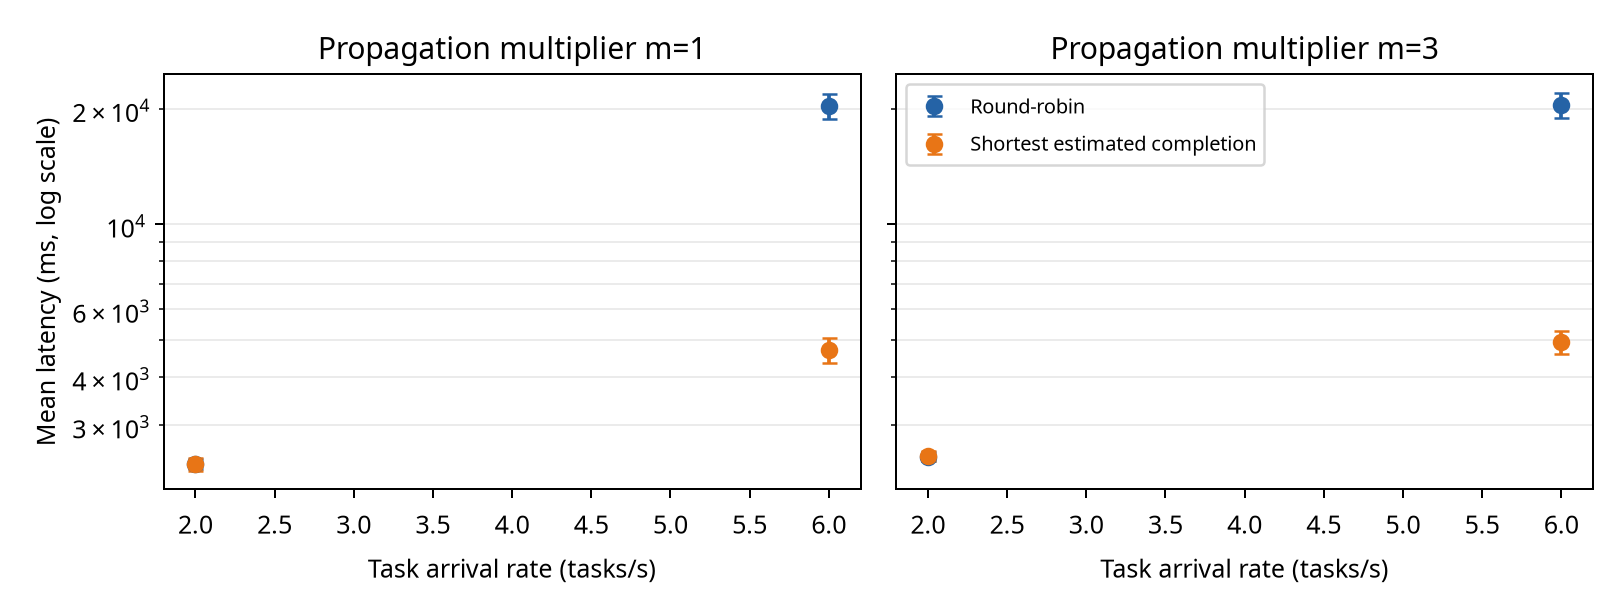
\includegraphics[width=0.85\textwidth]{extended_plot.png}
\caption{Mean end-to-end latency for RR and SEC in the event-driven model with 100-Mbit/s full-duplex access links. Error bars show 95\% t confidence intervals across replication-level means; the vertical axis is logarithmic.}
\label{fig:latency}
\end{figure*}

At $\lambda=6$ tasks/s and $m=1$, the mean of the replication-level p95 latencies is 64.1 s for RR and 8.65 s for SEC. This tail comparison is also configuration-specific and reflects the finite arrival cohort and unbounded queues.

\subsection{Offered load under Round-Robin}
Under RR each node receives one third of the tasks, so the offered utilization of a resource is $\rho=\lambda\,\bar{w}/(3C)$, where $\bar{w}$ is the mean demand per task and $C$ the capacity of that resource. Table~\ref{tab:rho} gives the values at $\lambda=6$ tasks/s, computed from the population means in Section~\ref{sec:model}. Edge\_1 and edge\_2 CPU pools and the edge\_2 uplink are offered more than their capacity ($\rho>1$), whereas the cloud is lightly loaded. At 2 tasks/s every resource has $\rho\le0.52$. The large high-load difference between RR and SEC is therefore consistent with RR saturating three resources during the 120-s window, and with SEC shifting about 54\% of tasks to the cloud (Section~\ref{sec:disc}). This is a property of capacity-blind dispatch in this parameterization, not evidence of a subtle SEC mechanism.

\begin{table}[t]
\caption{Offered Utilization $\rho$ Under RR at 6 Tasks/s (100-Mbit/s Access)}
\label{tab:rho}
\centering
\footnotesize
\begin{tabular}{lrrr}
\toprule
Resource & edge\_1 & edge\_2 & cloud\\
\midrule
CPU pool & 1.21 & 1.56 & 0.46\\
Node uplink & 0.72 & 1.15 & 0.29\\
Node downlink & 0.03 & 0.05 & 0.01\\
\bottomrule
\end{tabular}
\par\smallskip\raggedright Shared ingress: 0.86; shared egress: 0.08 (all policies).
\end{table}

\subsection{Access-capacity sensitivity}
Table~\ref{tab:access} shows that access capacity strongly changes both absolute latency and the relative policy difference. The mean offered input traffic is approximately $6\times1.794\times8=86.1$ Mbit/s. At 50 Mbit/s, mean ingress demand exceeds nominal capacity; this finite-window experiment accumulates a large ingress backlog, and SEC's relative reduction is only 1.8\%, although SEC is better in all 20 replications. The paired differences in this overloaded case depart from normality (Shapiro--Wilk $p=0.0078$), so its $t$ interval should be interpreted cautiously; the percentile bootstrap interval [570.5, 1200.8] ms and Wilcoxon test ($p<2\times10^{-6}$) support the same positive direction. At 100 and 200 Mbit/s, the reductions are 76.9\% and 81.1\%. At 100 Mbit/s the mean offered input load is about 86\% of capacity; at 200 Mbit/s it is about 43\%. These are sensitivity results for specified synthetic conditions, not predictions for an actual access network.

\begin{table*}[t]
\caption{Access-Capacity Sensitivity at 6 Tasks/s and $m=1$; Both Directions Use the Listed Rate}
\label{tab:access}
\centering
\footnotesize
\resizebox{\textwidth}{!}{%
\begin{tabular}{rrrrrr}
\toprule
Access rate (Mbit/s) & RR (ms) & SEC (ms) & RR--SEC (ms) & Paired 95\% CI (ms) & Reduction\\
\midrule
50 & 48244.3 & 47375.8 & 868.5 & [517.8, 1219.3] & 1.8\%\\
100 & 20345.8 & 4707.5 & 15638.3 & [14265.1, 17011.5] & 76.9\%\\
200 & 19771.8 & 3744.6 & 16027.2 & [14628.4, 17426.0] & 81.1\%\\
\bottomrule
\end{tabular}%
}
\end{table*}

\section{Supplementary Policy Checks}
\label{sec:supp}
This section is separate from the main experiment and was added after the main results were known; it is therefore exploratory. It uses the same simulator, task streams, seeds, and 20 paired replications. Two further policies are evaluated. \emph{SEC-R} is SEC whose reservations for already-assigned jobs use population-mean work and output sizes instead of their exact values. It assumes that a task's input size is available at dispatch; unlike the original SEC, it uses mean work and output sizes for previously assigned tasks rather than their exact generated values. \emph{WRR} is a smooth weighted Round-Robin with fixed weights 9:7:24, proportional to the configured aggregate compute rates; it uses no queue state.

Table~\ref{tab:supp} lists mean latencies. SEC-R has lower sample mean latency than SEC in all six tested conditions. At 6 tasks/s and $m=1$, the paired mean difference (SEC minus SEC-R) is 604 ms (95\% CI [480, 729] ms); this post-hoc comparison suggests that the main SEC result does not depend on using exact work/output reservations for previously assigned tasks, but it does not establish that SEC-R is generally superior. WRR is better than SEC at 6 tasks/s (by 644 ms for $m=1$, CI [555, 734] ms, and in all 20 replications), and at 2 tasks/s as well (by 123 ms, CI [62, 185] ms, for $m=1$). Between WRR and SEC-R the paired interval includes zero at 100~Mbit/s with $m=1$ (SEC-R minus WRR: 40 ms, CI [$-56$, 136] ms) but not with $m=3$. WRR is also significantly better than RR at 2 tasks/s (by 130 ms for $m=1$, CI [88, 173] ms), where SEC and RR did not differ. Thus most of the SEC--RR gap in the main experiment reflects RR ignoring node heterogeneity, and in this model a static capacity-weighted policy captures at least as much of the gain as the dynamic mean-based estimate. WRR relies on knowing the nominal node capacities, and nothing here shows how it would behave under changing capacities or workloads.

\begin{table}[t]
\caption{Supplementary Policies: Mean Latency (ms), 20 Paired Replications}
\label{tab:supp}
\centering
\footnotesize
\begin{tabular}{rrrrrrr}
\toprule
$\lambda$ & $m$ & Mbit/s & RR & SEC & SEC-R & WRR\\
\midrule
2 & 1 & 100 & 2378.7 & 2371.6 & 2275.9 & 2248.2\\
2 & 3 & 100 & 2481.1 & 2491.9 & 2461.3 & 2388.4\\
6 & 1 & 100 & 20345.8 & 4707.5 & 4103.1 & 4063.1\\
6 & 3 & 100 & 20448.3 & 4935.8 & 4447.9 & 4203.2\\
6 & 1 & 50 & 48244.3 & 47375.8 & 46953.8 & 46764.5\\
6 & 1 & 200 & 19771.8 & 3744.6 & 3292.2 & 3143.5\\
\bottomrule
\end{tabular}
\end{table}

\section{Discussion}
\label{sec:disc}
The extended model gives a load-dependent result. At 2 tasks/s, mean latency is approximately 2.4--2.5 s for both policies, and paired intervals span zero. At 6 tasks/s, RR assigns equal task counts despite unequal node capacities, producing substantial queues at the less powerful edge nodes. SEC routes an average of about 54\% of tasks to cloud at this load, versus 33.3\% under RR, shifting work toward the highest-capacity resource. This supports a conditional advantage over RR under high load, not a general claim that SEC always outperforms RR; moreover, the supplementary check shows that a static weighted RR does at least as well here, so the result should be read as a cost of capacity-blind dispatch rather than a merit specific to SEC.

The shared-link sensitivity shows that the bottleneck can move. With 50-Mbit/s ingress, offered input load exceeds capacity and dominates latency for both policies; changing placement then provides only a small relative improvement. At higher access rates, compute allocation has more influence and the measured advantage of SEC grows. The experiment varies ingress and egress together and does not independently attribute effects to each direction.

\section{Limitations and Threats to Validity}
First, node, core, and network parameters are illustrative and have not been calibrated against measurements from a physical system. Task sizes are synthetic and not drawn from real application traces. Second, the shared links are symmetric, full-duplex, unbounded FCFS queues carrying payload only; actual networks may have asymmetric bandwidth, cross traffic, finite buffers, protocol overhead, packet-level effects, or other queue disciplines. Third, the CPU model uses homogeneous cores within each node, one core per task, and no preemption or parallel task execution; cloud cores (300~MI/s) are slower per core than edge cores (450 and 350~MI/s), so the cloud's advantage comes only from core count, which is unusual in practice.

Fourth, SEC uses average sizes for an incoming task and assignment-time tail reservations for queues; prediction errors are expected, and actual event ordering can differ, particularly in multicore service. Fifth, the arrival window is finite and queues are drained after arrivals stop. Overloaded runs therefore report finite-cohort latency, not stationary performance under an infinite stream. Finally, 20 paired replications quantify only between-run variability. The baselines are limited to RR, SEC, and the two exploratory variants of Section~\ref{sec:supp}; no queue-length-based or randomized-choice policy was evaluated. Software tests and consistency checks do not validate the model against a real deployment.

\section{Conclusion}
This paper compared RR and a mean-based SEC heuristic in an event-driven edge--cloud simulation with shared full-duplex access links, node-specific links, propagation jitter, and multicore CPU pools. Under low arrival rate, no consistent difference was detected. At 6 tasks/s and 100-Mbit/s shared access, SEC reduced mean latency by 75.9--76.9\% across the two propagation settings. Under the high-load access-capacity sensitivity, the reduction ranged from 1.8\% at 50 Mbit/s to 81.1\% at 200 Mbit/s, illustrating that a congested common ingress can dominate placement effects. A supplementary comparison indicates that a static capacity-weighted Round-Robin performs at least as well as SEC at 6 tasks/s, so the large gap mainly reflects the cost of capacity-blind cyclic dispatch under overload of the edge resources.

The results support only a conditional conclusion for this synthetic model. They do not establish universal algorithmic superiority, global optimality, or real-world performance gains. Future work should calibrate the simulator with measured infrastructure and real traces, validate queue and network assumptions, compare additional policies, and study tail latency and scheduler overhead.

\begin{thebibliography}{7}
\bibitem{sonmez2018} C. Sonmez, A. Ozgovde, and C. Ersoy, ``EdgeCloudSim: An Environment for Performance Evaluation of Edge Computing Systems,'' \emph{Transactions on Emerging Telecommunications Technologies}, vol. 29, no. 11, Art. no. e3493, 2018, doi: 10.1002/ett.3493.
\bibitem{gupta2017} H. Gupta, A. V. Dastjerdi, S. K. Ghosh, and R. Buyya, ``iFogSim: A Toolkit for Modeling and Simulation of Resource Management Techniques in the Internet of Things, Edge and Fog Computing Environments,'' \emph{Software: Practice and Experience}, vol. 47, no. 9, pp. 1275--1296, 2017, doi: 10.1002/spe.2509.
\bibitem{zhang2022} Y. Zhang, B. Tang, J. Luo, and J. Zhang, ``Deadline-Aware Dynamic Task Scheduling in Edge--Cloud Collaborative Computing,'' \emph{Electronics}, vol. 11, no. 15, Art. no. 2464, 2022, doi: 10.3390/electronics11152464.
\bibitem{dreibholz2023} T. Dreibholz and S. Mazumdar, ``Towards a Lightweight Task Scheduling Framework for Cloud and Edge Platform,'' \emph{Internet of Things}, vol. 21, Art. no. 100651, 2023, doi: 10.1016/j.iot.2022.100651.
\bibitem{calheiros2011} R. N. Calheiros, R. Ranjan, A. Beloglazov, C. A. F. De Rose, and R. Buyya, ``CloudSim: A Toolkit for Modeling and Simulation of Cloud Computing Environments and Evaluation of Resource Provisioning Algorithms,'' \emph{Software: Practice and Experience}, vol. 41, no. 1, pp. 23--50, 2011, doi: 10.1002/spe.995.
\bibitem{eager1986} D. L. Eager, E. D. Lazowska, and J. Zahorjan, ``Adaptive Load Sharing in Homogeneous Distributed Systems,'' \emph{IEEE Transactions on Software Engineering}, vol. SE-12, no. 5, pp. 662--675, 1986, doi: 10.1109/TSE.1986.6312961.
\bibitem{mitzenmacher2001} M. Mitzenmacher, ``The Power of Two Choices in Randomized Load Balancing,'' \emph{IEEE Transactions on Parallel and Distributed Systems}, vol. 12, no. 10, pp. 1094--1104, 2001, doi: 10.1109/71.963420.
\end{thebibliography}
\end{document}
